\documentclass{beamer}
\usetheme{Montpellier}

\usepackage{color}
\usepackage{amsfonts}
\usepackage{comment}

%%% Al parecer necesito esto en ubuntu para los acentos
%\usepackage[spanish]{babel}
%\selectlanguage{spanish}
%\usepackage[utf8]{inputenc}

\definecolor{myblue}{rgb}{0.25, 0, 0.75}
\definecolor{mygold}{rgb}{1,0.8,0.2}
\definecolor{gray}{rgb}{0.5, 0.5, 0.5}
\definecolor{lucia}{rgb}{0.8,0.4,0.7} 

\newcommand{\myurl}[1]{\href{http://#1}{\textcolor{gray}{\texttt{#1}}}}
\newcommand{\myem}[1]{\structure{#1}}
\newcommand{\myurlshort}[2]{\href{http://#1}{\textcolor{gray}{\textsf{#2}}}}

\newcommand{\RPackage}[1]{\textcolor{gray}{\textsf{#1}}}
\newcommand{\pl}[1]{\texttt{#1}}
\newcommand{\RCode}[1]{\texttt{#1}}
\newcommand{\RFunction}[1]{\textsf{#1}}
\newcommand{\RClass}[1]{\textcolor{mygold}{\textsf{#1}}}
\newcommand{\BIOCfunction}[1]{\textcolor{orange}{#1}}

\setbeamercolor{example text}{fg=lucia}
\setbeamertemplate{sections/subsections in toc}[ball unumbered]
\setbeamertemplate{frametitle continuation}[from second][]
\setbeamertemplate{itemize subitem}[triangle]
\setbeamertemplate{footline}[page number]
\setbeamertemplate{caption}[numbered]
\setbeamertemplate{navigation symbols}{}

\renewcommand{\footnotesize}{\fontsize{6.10}{12}\selectfont}

\def\argmax{\operatornamewithlimits{arg\,max}}
\def\argmin{\operatornamewithlimits{arg\,min}}

%%\bibliographystyle{plain}


\title{Seminar III: R/Bioconductor}
\author{Leonardo Collado Torres \\ lcollado@lcg.unam.mx \\  Bachelor in Genomic Sciences \\ \myurl{www.lcg.unam.mx/\string~lcollado/}}
\date{
August - December, 2009
}








\usepackage{Sweave}
\begin{document}

\begin{frame}[allowframebreaks]
  \titlepage
\end{frame}

\section*{Class outline}

\begin{frame}[allowframebreaks]
  \frametitle{Public Data}
  \tableofcontents[hideallsubsections]
\end{frame}

%%%%%%%%%%%%%%%%%%%%%%%%%%%%%%%%%%%%%%%%%%%%%%%%%%%%%%%%%%%%%%%%%%%%%%%%%%%
\section{Intro}

\begin{frame}[allowframebreaks, fragile]
  \frametitle{To start off}
  \begin{itemize}
  \item On this class we'll learn how to download public data using tools such as \BIOCfunction{biomaRt}, \BIOCfunction{GEOquery} and \BIOCfunction{ArrayExpress}
  \item Please \alert{install} the following packages if you are working on your laptop.
\begin{Schunk}
\begin{Sinput}
> source("http://bioconductor.org/biocLite.R")
> biocLite(c("biomaRt", "GEOquery", 
+     "ArrayExpress"))
> biocLite(c("annotate", "KEGG.db", 
+     "KEGGSOAP"))
\end{Sinput}
\end{Schunk}
  \item You might need to install dependencies such as \pl{RCurl} and \pl{XML} for \pl{biomaRt}.
  \end{itemize}
\end{frame}

\begin{frame}[allowframebreaks]
  \frametitle{Why learn to use these packages?}
  \begin{itemize}
  \item Simply, because lots of data is publicly available.
  \item These tools help you avoid getting lost while fetching for data.
  \item Once the data is in \pl{R}\ldots graphs, statistical tests, etc.
  \end{itemize}
\end{frame}

\begin{frame}[allowframebreaks]
  \frametitle{Announcements}
  \begin{itemize}
  \item Assitance schedule defined:
  \begin{enumerate}
  \item Jos\'e on Tuesday 3 to 5
  \item V\'ictor on Wednesday 3 to 5
  \item Alejandro on Thursday 3 to 5
  \end{enumerate}
  \item Use Montealban preferably
  \item 1st homework :)
  \end{itemize}
\end{frame}


%%%%%%%%%%%%%%%%%%%%%%%%%%%%%%%%%%%%%%%%%%%%%%%%%%%%%%%%%%%%%%%%%%%%%%%%%%%
\section{biomaRt}

\begin{frame}[allowframebreaks]
  \frametitle{Intro}
  \begin{itemize}
  \item We'll dedicate most of the class to this package.
  \item Who is the author? He works with James Bullard :)
  \item There is a recent and very neat paper on \BIOCfunction{biomaRt} which uses other packages: \alert{lattice}, \alert{affy} and \alert{gplots}.
  \url{http://www.ncbi.nlm.nih.gov/pubmed/19617889}
  \end{itemize}
\end{frame}

\begin{frame}[allowframebreaks]
  \frametitle{What is biomart?}
  \url{http://www.biomart.org/}
  \begin{itemize}
  \item An \pl{OCR} and \pl{EBI} initiative.
  \item Access to 31 databases and \alert{growing}!\footnote{29 back in July 09}
  \item Not too hard to use :) You build a mart by choosing a database, some filters and you retrieve some attributes.
  \item Which databases do you find more \emph{interesting}?
  \end{itemize}
\end{frame}

\begin{frame}[allowframebreaks]
  \frametitle{ENSEMBL}
  \begin{itemize}
  \item One of the \BIOCfunction{biggest} public databases!
  \item Genes, GOs, regions, expression info, proteins, etc.
  \item If you want to learn more, take a look at the \myurlshort{www.ensembl.org/info/website/tutorials/index.html}{tutorials} site.
  \item Pay attention to Module 5: BioMart and the BioMart section :)
  \end{itemize}
\end{frame}

\begin{frame}[allowframebreaks]
  \frametitle{InterPro}
  \begin{itemize}
  \item \alert{Huge} one as well!
  \item Integrates data from several databases.
  \item Taxonomy, proteins, \ldots
  \item More info at the \myurlshort{www.ebi.ac.uk/interpro/}{InterPro} and the \myurlshort{www.ebi.ac.uk/interpro/mart_view_help.html}{mart help} sites.
  \end{itemize}
\end{frame}

\begin{frame}[allowframebreaks]
  \frametitle{biomaRt}
  \begin{itemize}
  \item Overall, BioMart is a web service tool to obtain tabular data.
  \item Is \BIOCfunction{biomaRt} the only way to access BioMart?
  \end{itemize}
\end{frame}

\begin{frame}[allowframebreaks, fragile]
  \frametitle{listMarts}
  \begin{itemize}
  \item \BIOCfunction{biomaRt} basically builds SQL queries for you and is more simple to use that doing the queries directly.
  \item To start, load the library and lets look at the available databases: \scriptsize
\begin{Schunk}
\begin{Sinput}
> library(biomaRt)
> head(listMarts())
\end{Sinput}
\begin{Soutput}
              biomart                                    version
1             ensembl               ENSEMBL 55 GENES (SANGER UK)
2                 snp          ENSEMBL 55 VARIATION  (SANGER UK)
3 functional_genomics ENSEMBL 55 FUNCTIONAL GENOMICS (SANGER UK)
4                vega                       VEGA 35  (SANGER UK)
5                 msd                     MSD PROTOTYPE (EBI UK)
6   bacterial_mart_54         ENSEMBL BACTERIA 54 GENES (EBI UK)
\end{Soutput}
\end{Schunk}
  \normalsize
  \end{itemize}
\end{frame}

\begin{frame}[allowframebreaks, fragile]
  \frametitle{Datasets}
  \begin{itemize}
  \item Once we know which \emph{mart} to use, we select it using \BIOCfunction{useMart}.
  \item Then, we can take a look at the available \alert{datasets}.
\begin{Schunk}
\begin{Sinput}
> mart <- useMart("bacterial_mart_54")
> head(listDatasets(mart))
\end{Sinput}
\begin{Soutput}
         dataset
1    str_57_gene
2    esc_20_gene
3 myc_25994_gene
4 sta_29522_gene
5     bac_6_gene
6 esc_31791_gene
                                  description
1 Streptococcus pneumoniae TIGR4 genes (EB 1)
2  Escherichia coli RIMD 0509952 genes (EB 1)
3        Mycobacterium bovis BCG genes (EB 1)
4      Staphylococcus aureus JH1 genes (EB 1)
5              Bacillus subtilis genes (EB 2)
6          Escherichia coli SE11 genes (EB 1)
  version
1    EB 1
2    EB 1
3    EB 1
4    EB 1
5    EB 2
6    EB 1
\end{Soutput}
\end{Schunk}
  \end{itemize}
\end{frame}

\begin{frame}[allowframebreaks, fragile]
  \frametitle{Filters}
  \begin{itemize}
  \item Now, we load the dataset with \BIOCfunction{useDataset} or we re-use \BIOCfunction{useMart} to subset our mart.
  \item And then we explore the available \alert{filters}.
\begin{Schunk}
\begin{Sinput}
> bsub <- useDataset("bac_6_gene", 
+     mart = mart)
> bsub <- useMart("bacterial_mart_54", 
+     dataset = "bac_6_gene")
> head(listFilters(bsub))
\end{Sinput}
\begin{Soutput}
                name
1    chromosome_name
2              start
3                end
4             strand
5 chromosomal_region
6  with_arrayexpress
              description
1         Chromosome name
2         Gene Start (bp)
3           Gene End (bp)
4                  Strand
5      Chromosome Regions
6 with ArrayExpress ID(s)
\end{Soutput}
\end{Schunk}
  \item A filter is our query, meaning, what we know.
  \item How many filters does our dataset have?
  \end{itemize}
\end{frame}

\begin{frame}[allowframebreaks, fragile]
  \frametitle{Attributes}
  \begin{itemize}
  \item We also need to choose what we want to know: the \alert{attributes}.
\begin{Schunk}
\begin{Sinput}
> head(listAttributes(bsub))
\end{Sinput}
\begin{Soutput}
                   name
1       ensembl_gene_id
2 ensembl_transcript_id
3    ensembl_peptide_id
4           description
5       chromosome_name
6        start_position
            description
1       Ensembl Gene ID
2 Ensembl Transcript ID
3    Ensembl Protein ID
4           Description
5    Chromosome/plasmid
6       Gene Start (bp)
\end{Soutput}
\end{Schunk}
  \item How may attributes we could potentially retrieve on this case?
  \end{itemize}
\end{frame}

\begin{frame}[allowframebreaks]
  \frametitle{Class exercise}
  \begin{itemize}
  \item Using our \BIOCfunction{bsub} \pl{Mart} object, retrieve the genes from the first 100000pb on the Bacillus chromosome with \alert{getBM}\footnote{\pl{getBM} is the main \pl{biomaRt} function}.
  \item For every gene, get the start position, end position, strand, and \emph{status}.
  \item Then use \alert{lattice} and make a plot using \pl{xyplot} with one panel for every type of status, the start on the $x$ axis and the end on the $y$ axis. Plot the points with different colors for every strand.
  \end{itemize}
\end{frame}

\begin{frame}[allowframebreaks, fragile]
  \frametitle{Solution: getting the data}
  \begin{itemize}
  \item The tricky part is using a \pl{list} for the filter values; a must when using more than one filter.
\begin{Schunk}
\begin{Sinput}
> res <- getBM(attributes = c("start_position", 
+     "end_position", "strand", "status"), 
+     filters = c("start", "end"), 
+     values = list("1", "100000"), 
+     mart = bsub)
> head(res)
\end{Sinput}
\begin{Soutput}
  start_position end_position strand
1          43921        44799      1
2          64099        64635      1
3          40213        40653      1
4          55866        56159      1
5          25221        25766     -1
6          53183        53368      1
  status
1  KNOWN
2  KNOWN
3  KNOWN
4  KNOWN
5  KNOWN
6  KNOWN
\end{Soutput}
\end{Schunk}
  \item How many genes did we get?
  \end{itemize}
\end{frame}

\begin{frame}[fragile, allowframebreaks]
  \frametitle{Solution: plot}
\begin{Schunk}
\begin{Sinput}
> library(lattice)
> print(xyplot(end_position ~ start_position | 
+     status, group = strand, data = res, 
+     auto.key = T))
\end{Sinput}
\end{Schunk}
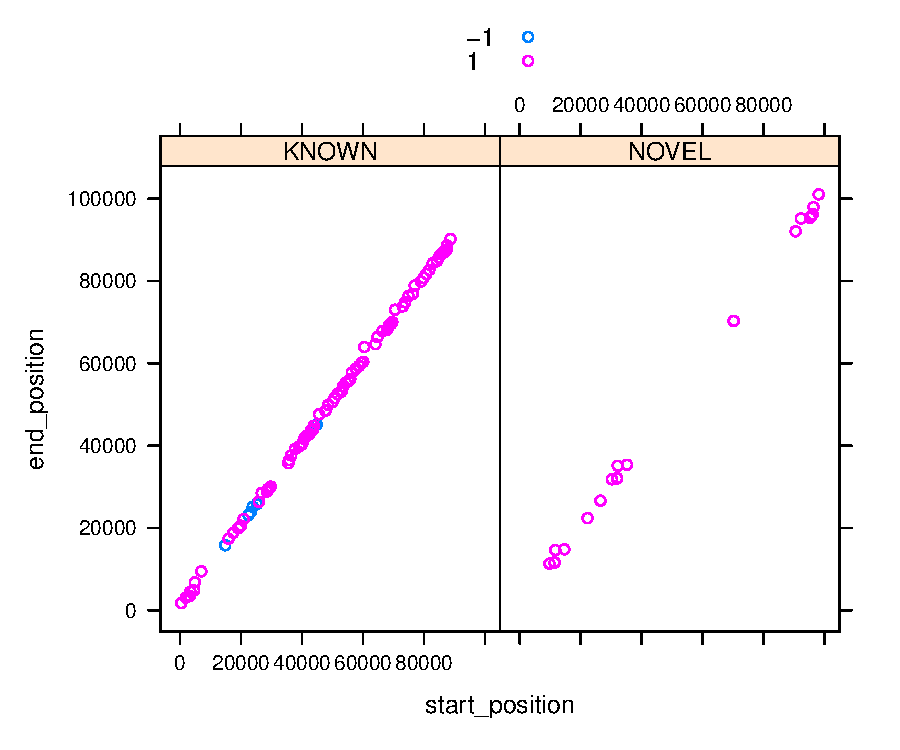
\includegraphics{plots/fig-010}
\end{frame}

\begin{frame}[allowframebreaks]
  \frametitle{Class Exercise II}
  \begin{itemize}
  \item Use \BIOCfunction{biomaRt} to access the Homo Sapiens dataset from the \pl{ENSEMBL} database.
  \item For \pl{entrez} gene ids 999, 1000 and 1001 get the first 100 upstream bases.
  \item Use the \BIOCfunction{getSequence} function.
  \item Set the \pl{seqType} argument equal to \emph{coding\_gene\_flank}.
  \item What is the GC percentage for every upstream sequence? Use \alert{gsub} and \alert{nchar}.\footnote{The answer is 72, 80, and 75}
  \end{itemize}
\end{frame}

\begin{frame}[allowframebreaks]
  \frametitle{For further learning}
  \begin{itemize}
  \item The \BIOCfunction{biomaRt} vignette is quite complete and presents several \emph{tasks} which are great for learning.
  \item Additionally, \myurlshort{www.stat.berkeley.edu/~steffen/}{Steffen} gave a lab at BioC2009 which has more tasks.
  \item Then again, the paper I mentioned earlier is quite elegant :)
  \end{itemize}
\end{frame}


%%%%%%%%%%%%%%%%%%%%%%%%%%%%%%%%%%%%%%%%%%%%%%%%%%%%%%%%%%%%%%%%%%%%%%%%%%%
\section{GEOquery}

\begin{frame}[allowframebreaks]
  \frametitle{Intro}
  \url{www.ncbi.nlm.nih.gov/geo/}
  \begin{itemize}
  \item \alert{GEO}, or the \pl{G}ene \pl{E}xpression \pl{O}mnibus, is a public data repository hosted at NCBI that mainly contains microarray data meeting MIAME requirements.
  \item There is some SAGE, mass spec data, and some high throughput data.
  \item \BIOCfunction{GEOquery} is simply the package to access this database from \pl{R}.\footnote{As far as I know, it doesn't work with HTS data for now}
  \end{itemize}
\end{frame}

\begin{frame}[allowframebreaks, fragile]
  \frametitle{Overview}
  \begin{itemize}
  \item The main function is \BIOCfunction{getGEO}.
\begin{Schunk}
\begin{Sinput}
> library(GEOquery)
\end{Sinput}
\end{Schunk}
\begin{Schunk}
\begin{Sinput}
> `?`(getGEO)
\end{Sinput}
\end{Schunk}
  \end{itemize}
\end{frame}

\begin{frame}[allowframebreaks, fragile]
  \frametitle{An example}
  \begin{itemize}
  \item As it says on the package help, \BIOCfunction{GEOquery} is the bridge between \pl{R} and \pl{GEO}.
  \item Lets look at some \myurlshort{www.ncbi.nlm.nih.gov/geo/query/acc.cgi?acc=GPL8251}{recent} data.
  \item Download the 2nd sample data.
\begin{Schunk}
\begin{Sinput}
> info <- getGEO("GSM377792")
\end{Sinput}
\begin{Soutput}
File stored at: 
/tmp/RtmpJTF9ag/GSM377792.soft
\end{Soutput}
\end{Schunk}
  \item Then check the attributes of our \pl{info} object
\begin{Schunk}
\begin{Sinput}
> attributes(info)
\end{Sinput}
\end{Schunk}
  \end{itemize}
\end{frame}

\begin{frame}[allowframebreaks]
  \frametitle{Cont.}
  \begin{itemize}
  \item What was it last updated?
  \item What organism did they study?
  \item What type of data is it?
  \item How old?
  \item Tissue type?
  \item Number of unique tags?
  \end{itemize}
\end{frame}

\begin{frame}[allowframebreaks]
  \frametitle{More info}
  \begin{itemize}
  \item You might want to save the data on a non-temp folder. To do so use the \BIOCfunction{destdir} arg.
  \item GDS data can be transformed into expression sets.
  \item If you work with microarrays, this package will be \emph{very} useful to you :)
  \end{itemize}
\end{frame}

%%%%%%%%%%%%%%%%%%%%%%%%%%%%%%%%%%%%%%%%%%%%%%%%%%%%%%%%%%%%%%%%%%%%%%%%%%%
\section{ArrayExpress}

\begin{frame}[allowframebreaks]
  \frametitle{Intro}
  \url{www.ebi.ac.uk/microarray-as/ae/}
  \begin{itemize}
  \item It's another public repository for public functional genomics data.
  \item Quite a few microarrays as well
  \end{itemize}
\end{frame}

\begin{frame}[allowframebreaks, fragile]
  \frametitle{Querying}
  \begin{itemize}
  \item First of all, you might want to look up for related data sets.
  \item We can do so using \BIOCfunction{queryAE}:\footnote{Note the use of a $+$ for multiple words}
\begin{Schunk}
\begin{Sinput}
> library(ArrayExpress)
> sets = queryAE(keywords = "pneumonia", 
+     species = "homo+sapiens")
\end{Sinput}
\end{Schunk}
  \item How many sets did we get? Check the \pl{class} of \pl{sets} first.
  \item When were multiple sets released the same day? We know that a \pl{unique} function exists, so using \BIOCfunction{apropos} find out the quickest solution :)
  \end{itemize}
\end{frame}

\begin{frame}[allowframebreaks, fragile]
  \frametitle{ArrayExpress}
  \begin{itemize}
  \item Once you identify the set you want to download, you can get it with \BIOCfunction{ArrayExpress}
  \item Note that one of its arguments is useful if you don't want to lose the data once you close the \pl{R} session.
\begin{Schunk}
\begin{Sinput}
> rawset = ArrayExpress("E-MEXP-1422")
\end{Sinput}
\end{Schunk}
  \item Around 15 mb of data on this case
  \end{itemize}
\end{frame}

\begin{frame}[allowframebreaks, fragile]
  \frametitle{Whole data}
  \begin{itemize}
  \item The previous function extracts some data from the array files, and if you want the whole data then you need to use \BIOCfunction{getAE}
\begin{Schunk}
\begin{Sinput}
> mexp1422 = getAE("E-MEXP-1422", 
+     type = "full")
\end{Sinput}
\end{Schunk}
  \end{itemize}
\end{frame}

\begin{frame}[allowframebreaks, fragile]
  \frametitle{Loading into \pl{R}}
  \begin{itemize}
  \item Once you have downloaded the files, you need to load them in \pl{R}.
  \item \BIOCfunction{magetab2bioc} does the job for you :)
\begin{Schunk}
\begin{Sinput}
> rawset = magetab2bioc(files = mexp1422)
\end{Sinput}
\end{Schunk}
  \item On this case, \pl{rawset} will be an \pl{AffyBatch} object.
  \item For processed data, you'll need to use \BIOCfunction{procset}.
  \end{itemize}
\end{frame}

\begin{frame}[allowframebreaks]
  \frametitle{We'll be back}
  \begin{itemize}
  \item We'll most likely re-use \pl{GEOquery} and \pl{ArrayExpress} on our microarray related classes.
  \end{itemize}
\end{frame}


%%%%%%%%%%%%%%%%%%%%%%%%%%%%%%%%%%%%%%%%%%%%%%%%%%%%%%%%%%%%%%%%%%%%%%%%%%%
\section{annotate}

\begin{frame}[allowframebreaks, fragile]
  \frametitle{Intro}
  \begin{itemize}
  \item Great to interact with NCBI!
  \item It uses \pl{XML} heavily
  \item You can download info on papers, sequences, make links to NCBI and much more :)
  \item There is a \alert{drawback}\ldots if you access NCBI too frequently you'll get banned.
  \end{itemize}
\end{frame}

\begin{frame}[allowframebreaks, fragile]
  \frametitle{Getting a sequence}
  \begin{itemize}
  \item For example, we can download sequences as \pl{character} objects using \BIOCfunction{getSEQ}
\begin{Schunk}
\begin{Sinput}
> library(annotate)
\end{Sinput}
\end{Schunk}
\begin{Schunk}
\begin{Sinput}
> seq <- getSEQ("CY045495.1")
\end{Sinput}
\end{Schunk}
  \item How long is our \pl{seq} object?
  \end{itemize}
\end{frame}

\begin{frame}[allowframebreaks, fragile]
  \frametitle{NCBI links}
  \begin{itemize}
  \item For \pl{getSEQ} I used a accession number, and if we want to find the related UID, simply use \BIOCfunction{accessionToUID}.
  \item Then, we can construct a link to NCBI using \BIOCfunction{getQueryLink}
\begin{Schunk}
\begin{Sinput}
> id <- accessionToUID("CY045495.1")
> id
\end{Sinput}
\begin{Soutput}
[1] "257127071"
\end{Soutput}
\begin{Sinput}
> getQueryLink(id, repository = "gb")
\end{Sinput}
\begin{Soutput}
[1] "http://www.ncbi.nlm.nih.gov/entrez/query.fcgi?db=Nucleotide&cmd=search&term=257127071"
\end{Soutput}
\end{Schunk}
  \item Where did our sequence come from?\footnote{Check the \pl{definition}}
  \item Does the length of \pl{seq} match the reported length?
  \item Find a way to get the NCBI link by using the accession number directly.
  \end{itemize}
\end{frame}

\begin{frame}[allowframebreaks, fragile]
  \frametitle{Paper info}
  \begin{itemize}
  \item By using the functions \BIOCfunction{pubmed}, \BIOCfunction{xmlRoot} and \BIOCfunction{buildPubMedAbst} we can get info such as abstracts, authors, \ldots
  \item Lets find the authors of our \pl{sets} object from the \pl{ArrayExpress} section.
\begin{Schunk}
\begin{Sinput}
> ids <- (sets[, "PubmedID"])
> ids <- as.character(ids[ids != 
+     "NA"])
> x <- pubmed("19679224")
> a <- xmlRoot(x)
> abs <- buildPubMedAbst(a[[1]])
\end{Sinput}
\end{Schunk}
  \item Once we have our \pl{abs} object\footnote{Note that I only built the abstract for the 1st paper}, we can retrieve information using its \alert{attributes}.
\begin{Schunk}
\begin{Sinput}
> pubDate(abs)
\end{Sinput}
\begin{Soutput}
[1] "Aug 2009"
\end{Soutput}
\end{Schunk}
  \item How many authors does the first paper have?
  \end{itemize}
\end{frame}

\begin{frame}[allowframebreaks]
  \frametitle{End}
  \begin{itemize}
  \item By using \pl{annotate}, its relatively easy to query abstracts for a gene name or some other keyword.
  \item I encourage you to explore it :)
  \end{itemize}
\end{frame}

%%%%%%%%%%%%%%%%%%%%%%%%%%%%%%%%%%%%%%%%%%%%%%%%%%%%%%%%%%%%%%%%%%%%%%%%%%%
\section{KEGG}

\begin{frame}[allowframebreaks, fragile]
  \frametitle{Quick overview}
  \url{www.genome.jp/kegg/kegg2.html}
  \begin{itemize}
  \item Finally, we'll take a very quick look at the \BIOCfunction{KEGG} packages.
\begin{Schunk}
\begin{Sinput}
> library(KEGG.db)
> library(KEGGSOAP)
> apropos("KEGG")
\end{Sinput}
\begin{Soutput}
 [1] "KEGG"                       
 [2] "KEGG2heatmap"               
 [3] "KEGG_dbconn"                
 [4] "KEGG_dbfile"                
 [5] "KEGG_dbInfo"                
 [6] "KEGG_dbschema"              
 [7] "KEGGENZYMEID2GO"            
 [8] "KEGGEXTID2PATHID"           
 [9] "KEGGGO2ENZYMEID"            
[10] "KEGGMAPCOUNTS"              
[11] "KEGGmnplot"                 
[12] "KEGGPATHID2EXTID"           
[13] "KEGGPATHID2NAME"            
[14] "KEGGPATHNAME2ID"            
[15] ".__M__KEGG2heatmap:annotate"
[16] ".__M__KEGGmnplot:annotate"  
[17] ".__T__KEGG2heatmap:annotate"
[18] ".__T__KEGGmnplot:annotate"  
\end{Soutput}
\end{Schunk}
  \item What is the name for the Path id 00010?
  \end{itemize}
\end{frame}

\begin{frame}[allowframebreaks, fragile]
  \frametitle{Quick answer}
  \begin{itemize}
  \item Easy, just use \BIOCfunction{KEGGPATHID2NAME}:
\begin{Schunk}
\begin{Sinput}
> KEGGPATHID2NAME$"00010"
\end{Sinput}
\begin{Soutput}
[1] "Glycolysis / Gluconeogenesis"
\end{Soutput}
\end{Schunk}
  \end{itemize}
\end{frame}

\begin{frame}[allowframebreaks, fragile]
  \frametitle{Genes}
  \begin{itemize}
  \item Next, if we want to find the genes involved on a certain pathway, we use \BIOCfunction{get.genes.by.pathway}\footnote{quite a long name!}
\begin{Schunk}
\begin{Sinput}
> genes <- get.genes.by.pathway("path:eco00010")
\end{Sinput}
\end{Schunk}
  \item How many genes did we get?
  \item For a deeper learning use:
\begin{Schunk}
\begin{Sinput}
> help(package = KEGGSOAP)
> help(package = KEGG.db)
\end{Sinput}
\end{Schunk}
  \end{itemize}
\end{frame}

\begin{frame}[allowframebreaks, fragile]
  \frametitle{SessionInfo} \scriptsize
\begin{Schunk}
\begin{Sinput}
> sessionInfo()
\end{Sinput}
\begin{Soutput}
R version 2.10.0 Under development (unstable) (2009-07-25 r48998) 
i686-pc-linux-gnu 

locale:
 [1] LC_CTYPE=en_US.UTF-8      
 [2] LC_NUMERIC=C              
 [3] LC_TIME=en_US.UTF-8       
 [4] LC_COLLATE=en_US.UTF-8    
 [5] LC_MONETARY=C             
 [6] LC_MESSAGES=en_US.UTF-8   
 [7] LC_PAPER=en_US.UTF-8      
 [8] LC_NAME=C                 
 [9] LC_ADDRESS=C              
[10] LC_TELEPHONE=C            
[11] LC_MEASUREMENT=en_US.UTF-8
[12] LC_IDENTIFICATION=C       

attached base packages:
[1] stats     graphics  grDevices
[4] utils     datasets  methods  
[7] base     

other attached packages:
 [1] KEGGSOAP_1.19.1    
 [2] KEGG.db_2.3.0      
 [3] RSQLite_0.7-1      
 [4] DBI_0.2-4          
 [5] XML_2.6-0          
 [6] annotate_1.23.1    
 [7] AnnotationDbi_1.7.7
 [8] ArrayExpress_1.5.5 
 [9] GEOquery_2.9.4     
[10] RCurl_0.98-1       
[11] bitops_1.0-4.1     
[12] Biobase_2.5.5      
[13] lattice_0.17-25    
[14] biomaRt_2.1.0      

loaded via a namespace (and not attached):
[1] affy_1.23.5         
[2] affyio_1.13.3       
[3] grid_2.10.0         
[4] limma_2.19.2        
[5] preprocessCore_1.7.4
[6] SSOAP_0.4-6         
[7] xtable_1.5-5        
\end{Soutput}
\end{Schunk}
\end{frame}


\end{document}

